\chapter{Generative Adversarial Networks : Principles, strengths and limitations}
\label{chap:chapter1}

\begin{chapterabstract}
	In this chapter, we propose an overview	 of the Generative Adversarial Networks \cite{Goodfellow2014} framework, some of its theoretical interpretations, as well as some of its variations and applications. We discuss the different limitations of this approach and expose a trilemma between the quality of the generated samples, their diversity and the conditioning of the model. We then discuss the recent advances that have been made to overcome some of these limitations and propose a taxonomy of these advances using the aforementioned trilemma. Finally, we discuss the evaluation of generative models and the difficulties of evaluating the intrinsic quality of a generated sample.  We propose an overview of the different classical metrics and discuss their limitations.
\end{chapterabstract}

\minitoc

\section{Generative Adversarial Networks}

Generative Adversarial Networks (\GAN) \cite{Goodfellow2014} have been recently highlighted for their ability to generate photo-realistic images. By providing a simple framework for high-quality, high-dimensional generative modeling, they quickly found real-world applications ranging from the notorious "deepfakes" \cite{Vaccari2020} to image super-resolution \cite{Ledig2016}.

In this section, we will first propose an overview of generative modeling with deep neural networks. We will focus on the Generative Adversarial Networks framework, their training process  and some of their variants, especially their conditional and domain-transfer variants.

We will then outline some limitations of this framework and propose a formulation of these limitations in the form of a trilemma between the intrinsic quality of the generated samples, their diversity and the quality of the conditioning of the model. With this tool, we propose a taxonomy of the recent \GAN approaches and identify trends in these approaches.



\subsection{Deep generative modeling}

Generative modeling with deep neural networks has been a challenging task due to its fundamentally stochastic nature, which prevents the computation of gradients. Indeed, whereas a discrimination tries to predict the class $y$ of a sample $x \sim \px$, which is to model the conditional probability distribution $\pyx$, the purpose of a generative model is to provide a sampling mechanism over $\px$  the intrinsic distribution of the data. By nature, this sampling mechanism is stochastic and therefore cannot be directly learned through gradient descent.

To overcome this problem,  Generative Stochastic Networks\cite{Bengio2012b}  model instead a parameterized Markov chain which converges to a point of the learned distribution. It uses the ergodicity property to generate samples by consecutive sampling on a randomly chosen starting point. %TODO \CR{To extend}

Instead of directly modeling $\px$, Variational Auto-Encoders (\ac{VAE})\cite{Kingmaa} learns to model a deterministic mapping $\pgxz$. From this mapping, the generative model can be obtain through marginalization: $\pgx = \int \pz \pgxz dz$. It then defines a variational lower bound of the data likelihood and trains the model as an auto-encoder which inner representation is pushed towards being the parameters of a Gaussian distribution. To generate a sample from the trained model, a random vector is be sampled from this Gaussian distribution and mapped to the learned distribution by the decoder network.

%TODO \CR{Maybe add autoregressive models and flow-based models}

\subsection{The GAN framework}

In the same fashion, Generative Adversarial Networks aims to learn a parameterized mapping $\pgxz$ between a simple distribution $\pz$ (usually normal or uniform) to the real data distribution $\px$. However, instead of trying to estimate the distribution through marginalization and approximate inference, it aims to directly minimize an estimation of a divergence between $\px$ and the mapped distribution $\pgx$. 

However, because divergences are usually intractable, \GANs rely on a second learned function that will act as an adversary: the discriminator $\D$.  The discriminator is a binary classifier that aims to predict the probability that a sample $x$ was sampled on the real distribution $\px$ or was  generated from $z\sim\pz$ and is trained by minimizing the  binary cross-entropy. The objective of the generator $\G$ is then to fool the discriminator by maximizing the same binary cross-entropy. This training process is summed up as a mini-max game in \citeq{eq:GAN_problem} 

\begin{equation}
\label{eq:GAN_problem}
\arg\min_\G\max_\D\lgan = \arg\min_G\max_\D \esp{x\sim \px} [\log \D(x)] +  \esp{z\sim\pz} [1 - \log \D(\G(z))]
\end{equation}

This mini-max game has, assuming infinite capacity for both $G$ and $D$, a global optimum for $\px = \pgx$, which can be proved as follows: the minimum of $f(x) = a\log(x) + b\log(1-x)$ is $\frac{a}{a+b}$, the discriminator that maximizes the criterion for a fixed $\G$ is given by

\begin{equation}
\label{eq:optimal_D}
\D^*_\G(x) = \frac{\px}{\px + \pgx}
\end{equation}

We can formulate a criterion $C(\G)$ by plugin this optimal discriminator in \citeq{eq:GAN_problem}

\begin{align}
		C( \G) &= \max_\D\lgan(\D, \G) \nonumber\\
		& = \esp{x\sim \px} \Big[\log \D^*(x)] +  \esp{z\sim P_z} \Big[1 - \log \D^*(\G(z))\Big] \nonumber = \esp{x\sim \px} \Big[\log \D^*(x)\Big] +  \esp{{x}\sim \pgx} \Big[1 - \log \D^*(x)\Big] \nonumber \\
		& = \esp{x\sim \px} \Big[\log \frac{\px}{\px + \pgx}\Big] +   \esp{{x}\sim \pgx} \Big[1 - \log  \frac{\pgx}{\px + \pgx}\Big] \nonumber \\
\end{align}

Up to additive and multiplicative constants, the criterion  $C(\G)$ can be reformulated as

\begin{equation}
		C(\G) = \DKL \Big(\px\Big|\Big|\frac{\px+\pgx}{2} \Big) + \DKL \Big(\pgx \Big|\Big| \frac{\px+\pgx}{2} \Big) = 2\cdot\JSD \Big(\px\Big|\Big|\pgx \Big)
\end{equation}

When the discriminator is trained to convergence, minimizing the criterion $C( \G) = \lgan(\D^*, \G)$ is equivalent to minimizing the Jensen-Shannon (\ac{JS}) divergence between $\px$ and $\pgx$. The \GAN training process then consists in alternatively updating the discriminator and the generator via gradient ascent/descent. A summary of this process is presented in \citealg{alg:GAN_train}. 

\begin{algorithm}[!ht]
	\caption{The\GAN training algorithm}
	\label{alg:GAN_train}
	\begin{algorithmic}[H]
		\REQUIRE{$\trainsetX$ the real dataset, $G$ the generator model, and $D$ the discriminator model}
		\REPEAT
		\STATE sample a mini-batch $\lbrace x_i \rbrace_{i=1}^m$ from $\trainsetX$\;
		\STATE sample a mini-batch $\lbrace z_i \rbrace_{i=1}^m$ from $\pz$\;
		\STATE update $D$ by stochastic gradient ascent of
		\STATE \ \ \ \ $ \sum_{i=1}^{m}\log(D(x_i)) + \log(1-D(G(z_i)))$
		\STATE sample a a mini-batch $\lbrace z_j \rbrace_{j=1}^n$ from distribution $\pz$\;; 
		\STATE update $G$ by stochastic gradient descent of
		\STATE \ \ \ \ $ \sum_{j=1}^n \log(1-D(G(z_j)))$\;
		\UNTIL a stopping condition is met
		
	\end{algorithmic}
\end{algorithm}


\subsection{Conditional modeling with  \ac{CGAN}s}

While classical generative models such as \GANs try to unconditionally approximate the real-data distribution $\px$, a conditional generative model aim to learn a model of the conditional distribution $\pxy$, where $y \in \setY$ is a label of any kind.

Several extensions of the \GAN framework allow for conditional modeling. First introduced, Conditional \GANs (\ac{CGAN}s)\cite{Goodfellow2014}\cite{mirza17} simply adds the label $y$ as an input for both the discriminator and the generator. The new optimization problem that results from this change is summed-up in \citeq{eq:CGAN_problem} as follows

\begin{equation}
\label{eq:CGAN_problem}
		\arg\min_G\max_\D \lcgan = 	\arg\min_G\max_\D \esp{x,y\sim \pjxy} [\log \D(x, y)] +  \esp{y\sim \py \\ z\sim\pz} [1 - \log \D(\G(y, z), y)]
\end{equation}

While this approach is trivially simple to implement, it relies entirely on the discriminator to use the label. Other approaches try to learn the conditional distribution by adding an explicit loss term to the optimization problem, such as Auxillary Classifier GAN (\ac{ACGAN}) \cite{Odena}. This approach aims to learn a conditional generative model with discrete labels by adding another output to the discriminator that acts as a classifier. The model is then trained by having both the generator and the discriminator minimize the categorical cross-entropy  between the real and predicted labels.

\subsection{Domain-transfer with \GANs}

Domain-transfer is the task of learning a mapping $\pxy$ between two high-dimensional distributions $\px$ and $\py$ that maintains semantic information, for example changing the color palette of an image while keeping the same objects at the same position. \ac{CGAN}s already learn to model the conditional distribution $\pxy$, and adding a way to enforce the consistency of the semantic information enables
domain-transfer.

Pix2Pix \cite{Isola2016} implemented this approach  explicitly by using paired samples $(x, y) \sim \pxy$ forcing the generator to minimize the $\Lone$ reconstruction term between $x$ and $\G(y,z)$ (\citeq{ex:pix2pix}). 

\begin{equation}
\label{eq:pix2pix}
\arg\min_G\max_\D L_{p2p} =  \arg\min_G\max_\D \lcgan(\D, \G) +\lambda\esp{x\sim\px\\y\sim\py\\z\sim\pz} ||x - G(y, z)||_1
\end{equation}

However, this kind of approaches rely on paired data which can be very hard to obtain, especially in the case of natural images. When trying for example to transfer images of zebras to images of horses, you need a dataset of very similar zebras and horses in the exact same position for the $\Lone$ term to work.

This problem of paired data was solved by \ac{CycleGAN }\cite{Zhu} using cycle-consistency. Instead of training a single model $\G$ with reconstruction between $x$ and $\G(y,z)$, the CycleGAN approach train two domain-transfer models simultaneously: $\Gyx$ and $\Gxy$ that map samples from $\py$ onto $\px$ and $\px$ onto $\py$, respectively. This allows to compute the $\Lone$ reconstruction errors  $||x - \Gyx(\Gxy(x))||_1$ and $||y - \Gxy(\Gyx(y))||_1$, thus completely removing the need for paired data $(x,y)$. The training of the two models in done an adversarial setup, with two discriminators $\Dx$ and $\Dy$, and is summed up as an optimization problem in \citeq{eq:cyclegan}

\begin{align}
\label{eq:cyclegan}
\arg\min_{\Gxy, \Gyx}\max_{\Dx, \Dy} \lcycgan &=   \arg\min_{\Gxy, \Gyx}\max_{\Dx, \Dy} \lgan(\Dx, \Gyx) + \lgan(\Dy, \Gxy) \nonumber \\
& +\lambda \esp{x\sim\px} ||x - \Gyx(\Gxy(x)||_1 + \lambda\esp{y\sim\py} ||y - \Gxy(\Gyx(y)||_1
\end{align}

The \ac{CycleGAN} training process then consists in alternatively updating the two discriminator and the two generators via gradient ascent/descent. A summary of this process is presented in \citealg{alg:cyclegan_train}. 

\begin{algorithm}[]
	\begin{algorithmic}[H]
		\REQUIRE{$\setX$ and $\setY$ two unpaired datasets, $\Gxy$ and $\Gyx$ the mapping networks, $\Dx$ and $\Dy$ the discrimination models, $m$ the mini-batch size}
		\REPEAT
		\STATE sample a mini-batch $\lbrace x_i \rbrace_{i=1}^m$ from $\setX$\;
		\STATE sample a mini-batch $\lbrace y_i \rbrace_{i=1}^m$ from $\setY$\;
		\STATE update $\Dx$ by stochastic gradient descent of
		\STATE \ \ \ \ $ \sum_{i=1}^{m}(\Dx(x_i)-1)^2 + (\Dx(\Gyx(y_i)))^2$
		\STATE update $\Dy$ by stochastic gradient descent of
		\STATE \ \ \ \ $ \sum_{i=1}^{m}(\Dy(y_i)-1)^2 + (\Dy(\Gxy(x_i)))^2$
		\STATE sample a mini-batch $\lbrace x_i \rbrace_{i=1}^m$ from $X$\;
		\STATE sample a mini-batch $\lbrace y_i \rbrace_{i=1}^m$ from $Y$\;
		\STATE update $\Gxy$ by stochastic gradient descent of
		\STATE \ \ \ \ $ \sum_{i=1}^n (\Dy(\Gxy(x_i))-1)^2 + \lambda (||x_i - \Gyx(\Gxy(x_i))||_1$ \STATE \ \ \ \ \ \ \ \ $+||y_i -\Gxy(\Gyx(y_i))||_1)$\;
		\STATE update $\Gyx$ by stochastic gradient descent of
		\STATE \ \ \ \ $ \sum_{i=1}^n (\Dx(\Gyx(y_i))-1)^2+ \lambda (||x_i - \Gyx(\Gxy(x_i))||_1 $
		\STATE \ \ \ \ \ \ \ \ $+ ||y_i - \Gxy(\Gyx(y_i))||_1)$\;
		\UNTIL a stopping condition is met
	\end{algorithmic}
	\caption{CycleGAN training algorithm}
	\label{alg:cyclegan_train}
\end{algorithm}

\section{Limitations}

While \GANs have shown strong advantages over the classical generative modeling methods, such as generating sharper samples, they still exhibit limitations, namely: the instability of the training process; the diversity of the generated samples, the problem of \textit{mode-collapse}; and finally the problems due to conditioning. 

The instability of the \GAN training process has first been conjectured to be caused by the bad quality of the gradients obtained when $\G$ generates bad samples, which makes $\D$ strongly reject these samples and therefore saturating the loss. The first solution proposed \cite{Goodfellow2014} was to slightly change the generator's loss function from $\log(1-\D(\G(z)))$ to $-\log(\D(\G(z)))$, which helped considerably to avoid failures of the training process and was then widely used%TODO références.

 While this loss term converges to the same minimum as the original loss term, it however no longer correspond to a \ac{JSD}

\CR{
Image quality : Incremental enhancement through architecture, more data, ... 

Instability, catastrophic forgetting and the mode collapse problem

Trade-off image quality/diversity : Explanation through the loss term and distribution coverage

Black-box approach to conditioning, no tuning possible, no interpretability
}
\section{The GAN Zoo}

\subsection{A taxonomy of GANs}
Enorme nombre de variantes de GANs

Taxonomie des approches GANs (pour s'éviter une liste des différents GANs)

Schéma pour définir les grandes familles de GAN (évoquer les AmbientGAN / UNIR)

\subsection{Architecture variants}

\subsection{Divergence variants}
Table des loss alternatives (f-divergences + transport optimal)

\subsection{Task-specific losses}

\begin{figure}
	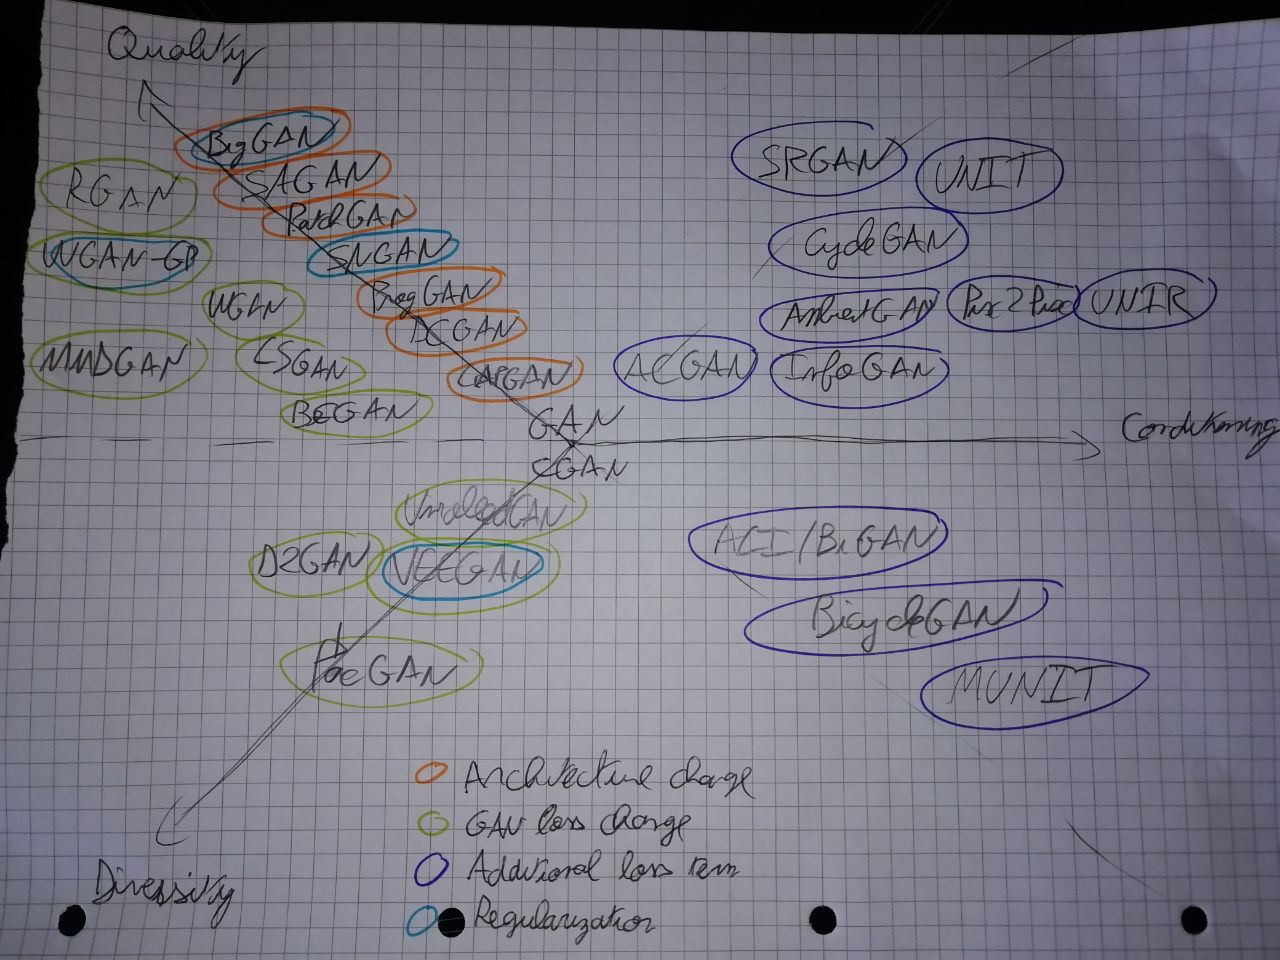
\includegraphics[width=\textwidth]{chapter1/trilemma.jpg}
	\caption{Classifications of some advances in GANs on the trilemma}
\end{figure}

\section{A note on the  evaluation of generative models}

No good adhoc methods

Image quality : Inception distance + Fréchet inception distance, advantages

Conditioning : Direct evaluation (pixel-wise), Classifier accuracy, Projections (PCA, t-SNE)

Limitations of those metrics : need a pre-trained model


